\documentclass[12pt]{report}
\usepackage{cmap}

\usepackage[T1]{fontenc}
\usepackage[utf8]{inputenc}

\usepackage[english]{babel}
%\usepackage[english,russian]{babel}

\usepackage{hyperref}

\usepackage{amsthm}
\usepackage{amsmath}
\usepackage{amssymb}
\usepackage{amsfonts}
\usepackage{amsthm}
\usepackage{enumerate}
%\usepackage{enumitem}
\usepackage{tikz}
\usepackage{xcolor}
\usepackage{textcomp}

\usepackage{listings}

\usepackage{comment}

\newcommand{\struct}[1]{\textcolor{blue}{#1}}
\newcommand{\Rim}[1]{\uppercase\expandafter{\romannumeral#1}}
\newcommand{\cmd}[1]{\textcolor{blue}{#1}}

\definecolor{mverb}{HTML}{C0E8F8}

\lstnewenvironment{code}[1]{%
  \lstset{backgroundcolor=\color{#1},
  frame=single,
  showlines=true,
  framerule=0pt,
  basicstyle=\ttfamily,
  columns=fullflexible}}{}

\title% (optional, use only with long paper titles)
{UNIX AND LINIX\\IN INFOCOMMUNICATION}

\author % (optional, use only with lots of authors)
{O.~Sadov%,\\ \texttt{tit@astro.spbu.ru}
}
% - Give the names in the same order as the appear in the paper.
% - Use the \inst{?} command only if the authors have different
%   affiliation.

%%%\institute{ITMO}
%  Университет Информационных Технологий, Механики и Оптики\\
%  кафедра Телекоммуникационных Систем

% - Use the \inst command only if there are several affiliations.
% - Keep it simple, no one is interested in your street address.

\date% (optional, should be abbreviation of conference name)
{1.09.2020}


\begin{document}
\maketitle

\section*{History}

\hbox{\begin{minipage}{0.80\textwidth}
\emph{\struct{{\Large If I have seen further than others,\\
it is by standing upon the shoulders of giants}}}\\
\mbox{}\hfill \emph{\struct{Isaac Newton}}
\end{minipage}\hspace{1em}
\begin{minipage}{0.15\textwidth}

\includegraphics[scale=0.3]{I_Newton.jpg}
\end{minipage}}

\medskip
This is a well-known saying.
But we must understand that many of these giants have failed.
But such fails can be a good lesson for new developers.

\medskip
\hbox{\begin{minipage}[b]{0.2\linewidth}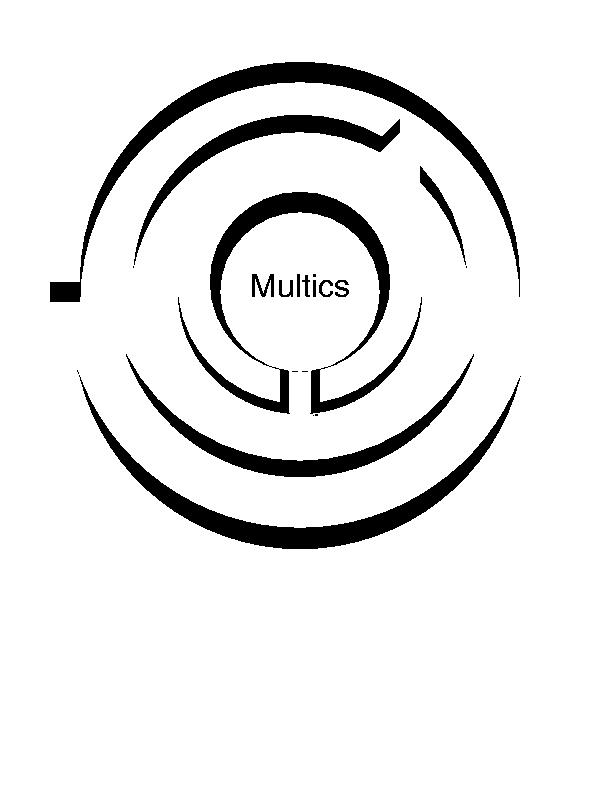
\includegraphics[scale=0.125]{Multics.png}
\end{minipage}
\begin{minipage}[b]{0.8\linewidth}
One such giant was the MULTICS project. The development of Multics began
in 1965 as a research project by MIT, General Electric and Bell Labs to create
a time-sharing, multiprocessing and multiuser interactive operating system.
After several years of development, the enthusiasm of the developers decreased
more and more as the system became more and more complex and the prospects
for completion of development became less and less.
\end{minipage}}

\medskip
\hbox{\begin{minipage}[b]{0.64\linewidth}
Bell Labs pulled out of the project in 1969; but some of the people
who worked on it got a lot of experience. Among them were \struct{Ken Thompson}
and \struct{Dennis Ritchie} of Bell Labs, the inventors of the \struct{UNIX OS}.
\end{minipage}\hspace{1em}
\begin{minipage}[b]{0.32\linewidth}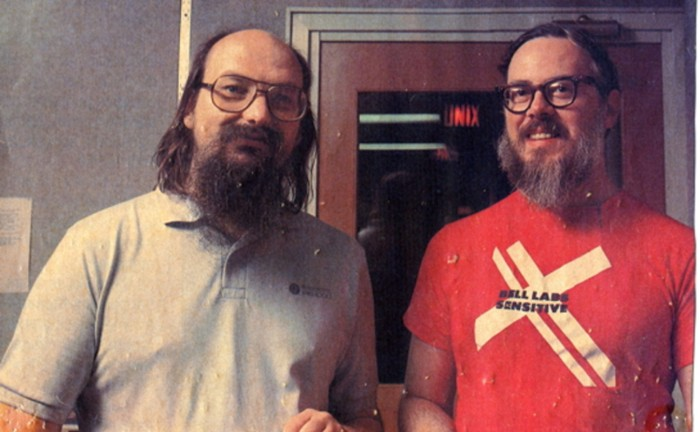
\includegraphics[scale=0.18]{thompson_ritchie.jpg}
\end{minipage}
}

\medskip
\hbox{\begin{minipage}[b]{0.5\linewidth}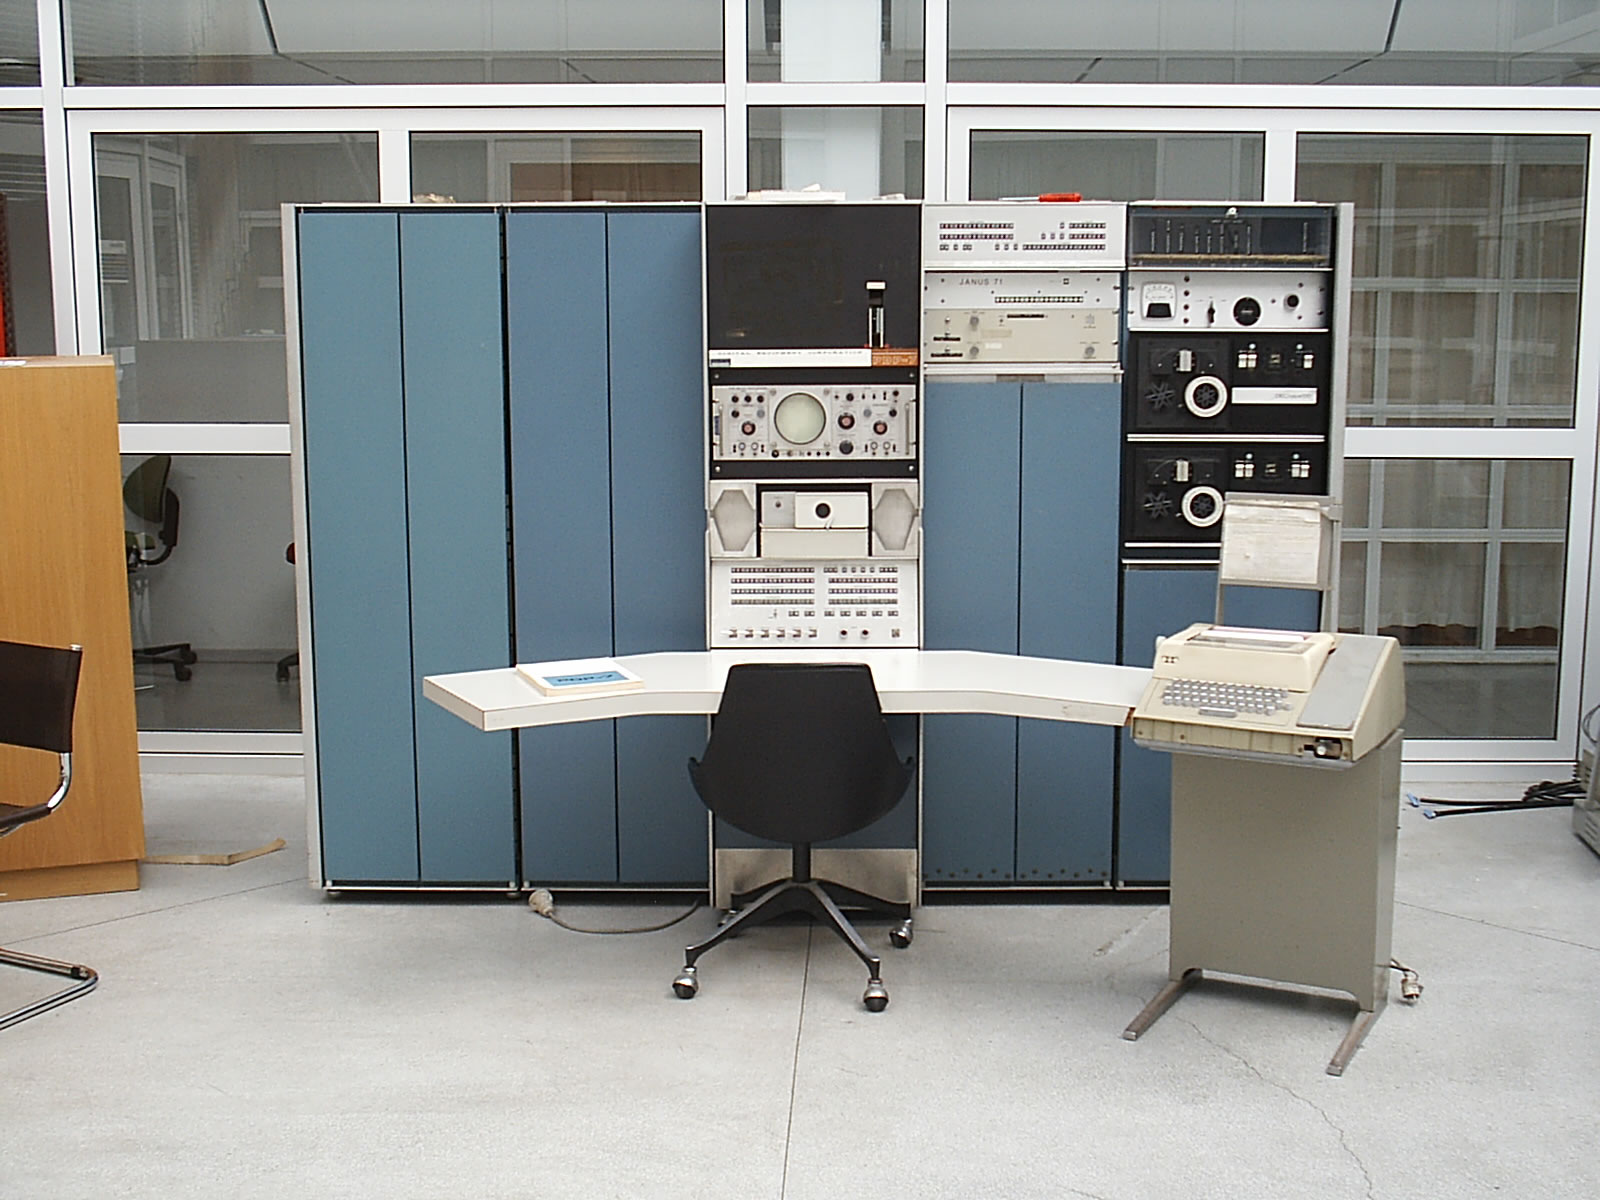
\includegraphics[scale=0.1]{Pdp7-oslo-2005.jpg}
\end{minipage}\hspace{1em}
\begin{minipage}[b]{0.5\linewidth}
It's funny, but the history of Unix systems is closely related to computer games.
It started in 1969 when Ken Thompson discovered an old \mbox{PDP-7} computer
in a dark corner of the lab and wanted to use it to play Space Travel game.\\\\
\end{minipage}
}

\medskip
There was little to do~--- an operating system had to be written to run it.
And he did it at 1970. It was originally a single-tasking OS written
in assembly language that was loaded from paper tapes and called UNICS
as opposed to the complexity of MULTICS.

\hbox{\begin{minipage}[b]{0.65\linewidth}
And then the team of Ken Thompson and Dennis Ritchie received a new DEC PDP11
computer to develop a word processing system for the Bell Labs patent department.
For the first three months the machine sat in a corner, enumerating all
the closed Knight's tours on a $8\times8$ chess board~---
just because the hard drive wasn't shipped with a super new computer.
This time could be used to choose a programming language, because it was
a computer with a completely new architecture and programs written on PDP7
assembler was not
\end{minipage}\hspace{1em}
\begin{minipage}[t]{0.35\linewidth}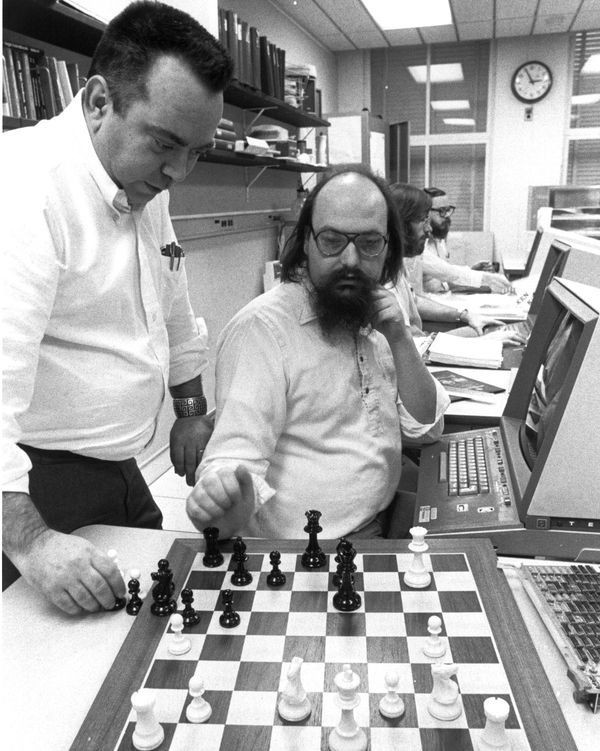
\includegraphics[scale=0.18]{chess.jpg}
\end{minipage}
}

\noindent
useful for it. And most interesting was the concept of another project used
in some R\&D projects including MULTICS~--- \struct{BCPL}.
It was a high-level programming language focused on portability.
Most of this language was written in the language itself, and only a small
machine-dependent part was written in assembly. To support a new machine,
only 1/5 of the compiler code needed to be rewritten, which usually took
2-5 man-months.

\medskip
Thompson used the same concept when writing his simplified successor to BCPL,
language \struct{B}. This language was not very expressive and effective on
the \struct{PDP11}. In 1972, Ritchie started to improve B, which resulted in
creating a new language \struct{C}. In 1973, the UNIX kernel was refactored
in C language to follow the same concept of portability~--- most of the code
was machine independent.
\begin{center}
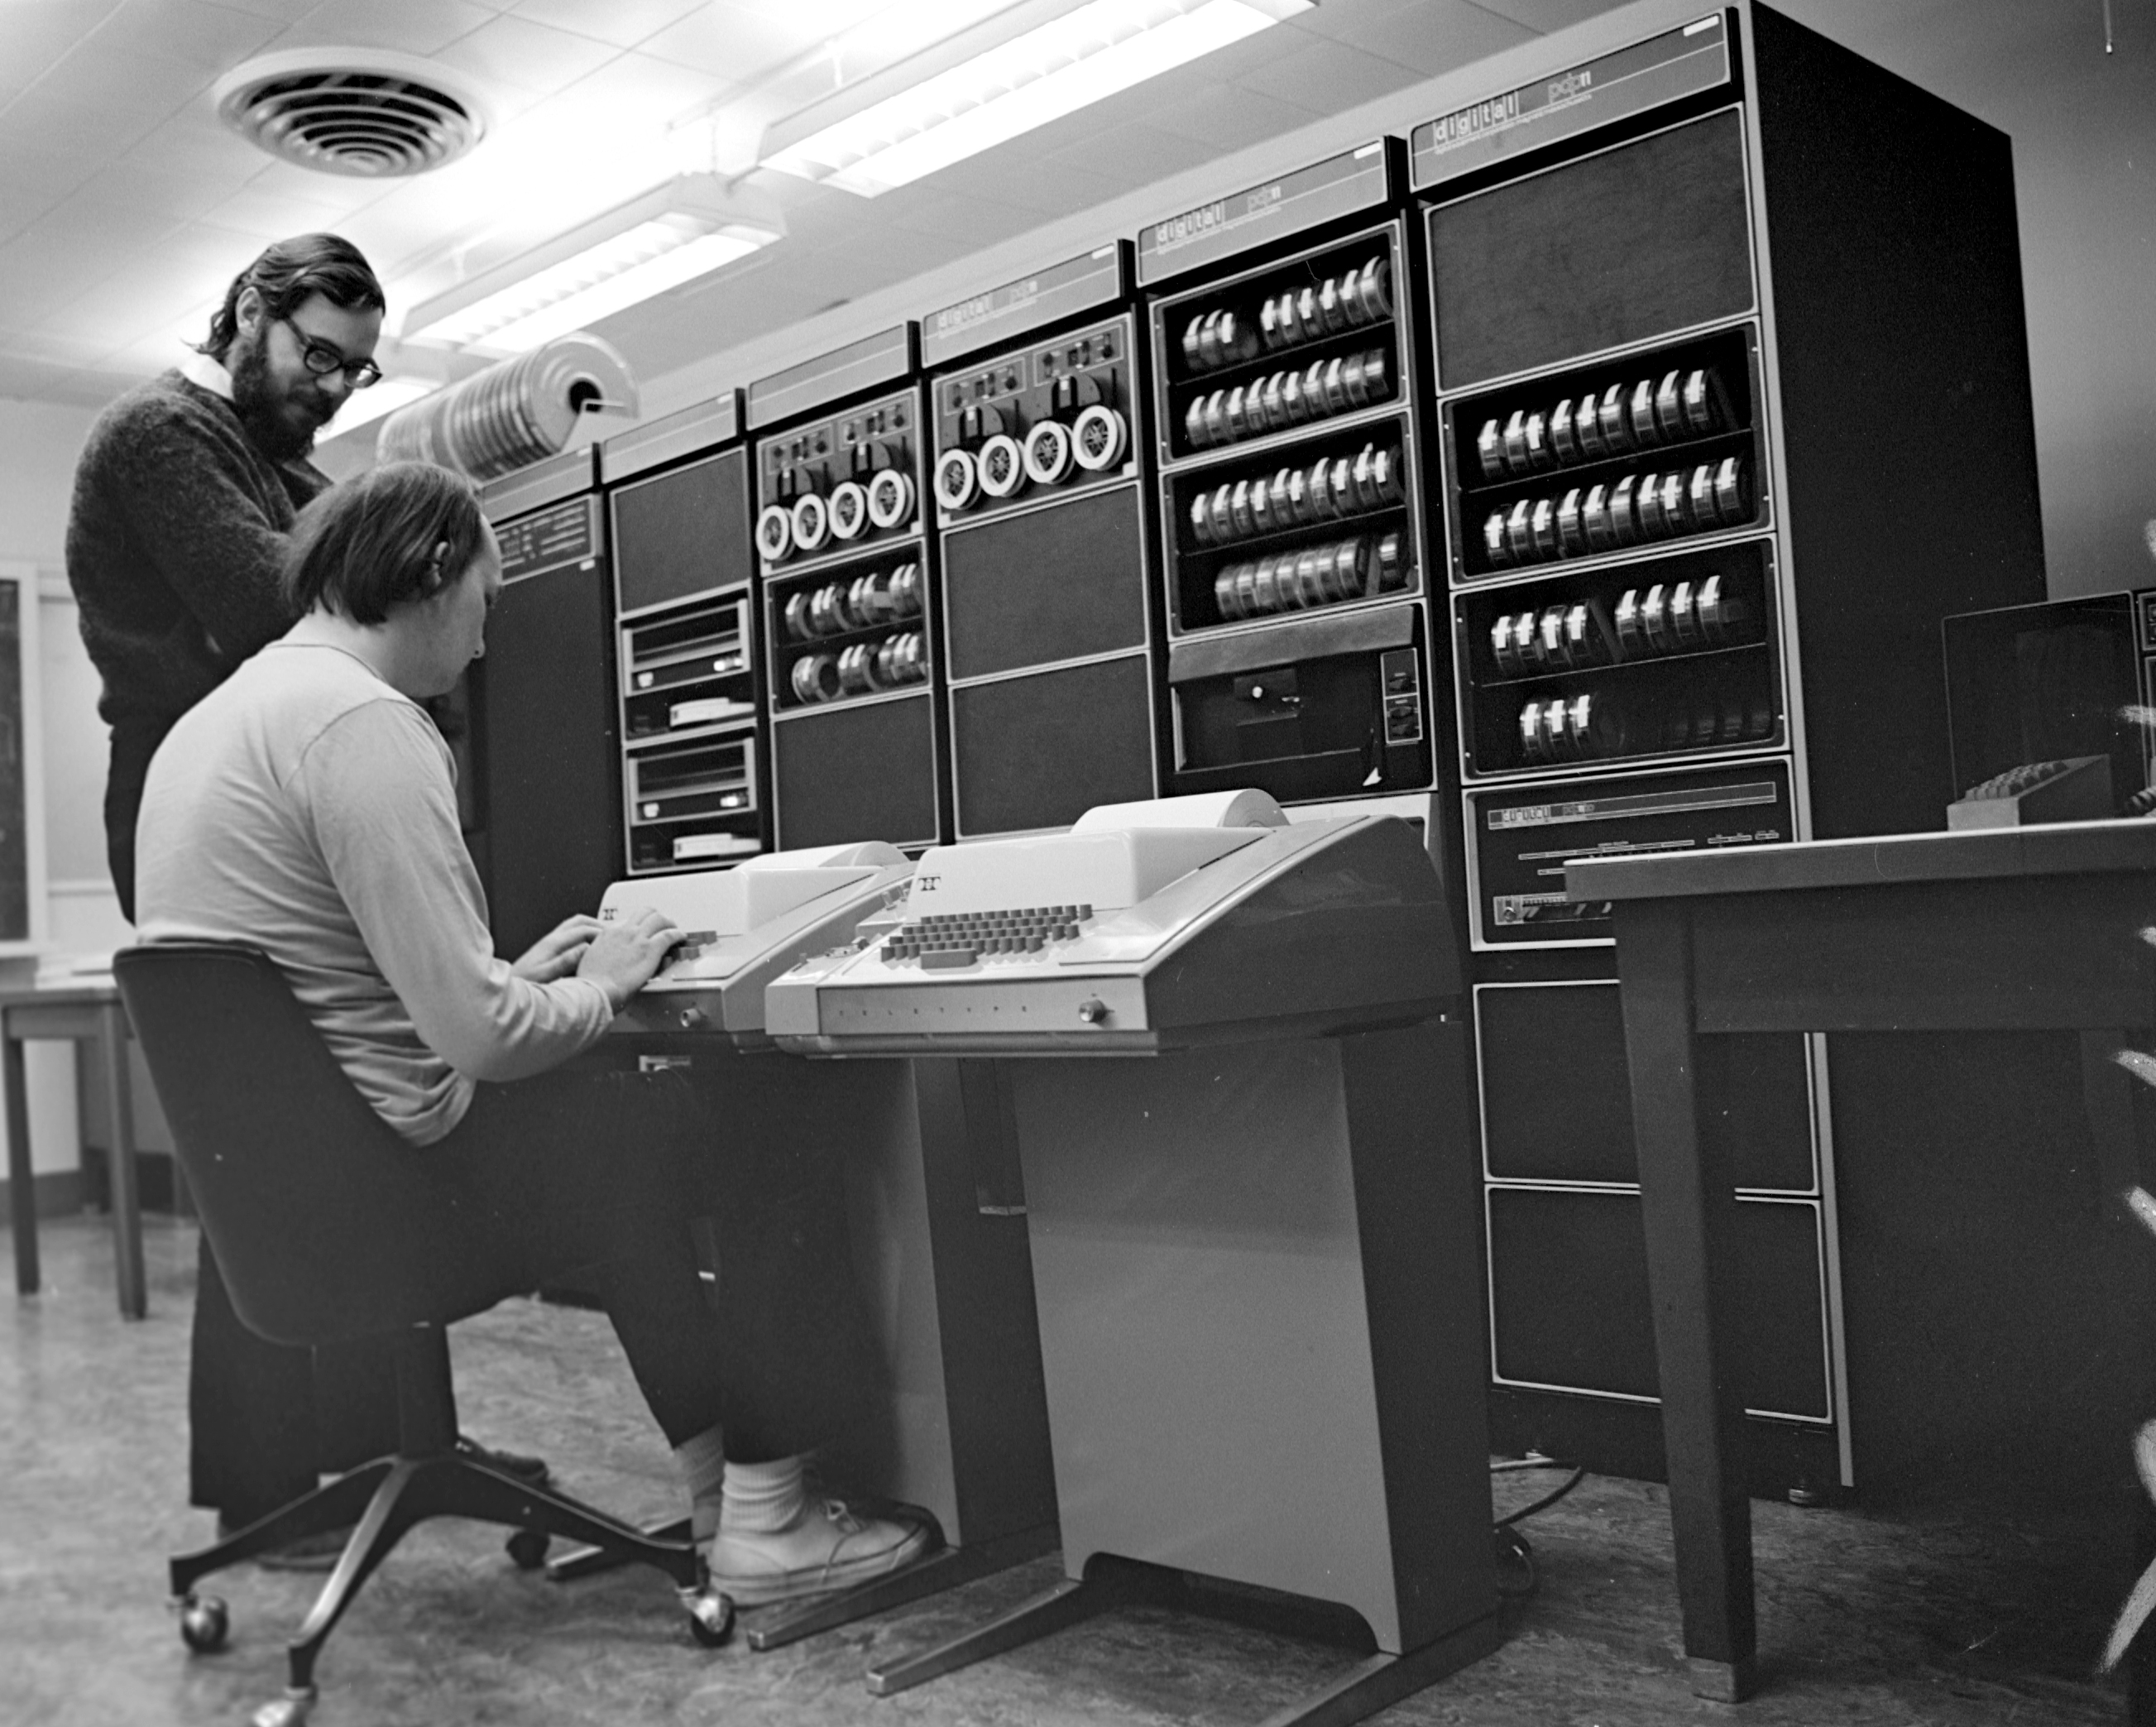
\includegraphics[scale=0.9]{Ken_Thompson__and_Dennis_Ritchie_at_PDP-11.jpg}
\end{center}
%Finally, they got a very flexible and powerful system with
%a rich set of applications.

\medskip
The system was distributed in source code among universities for a nominal fee,
which served as an explosive growth in its popularity in the 80s.
Almost all the developers of new computer systems since this period have used
UNIX as the base platform for their new developments. One of the most famous of
these is the Berkeley Software Distribution (\struct{BSD}) developed at
the University of California, Berkeley based on \struct{Unix version 6}
with its own \struct{copyleft license}. And most of the hardware vendors of
the 1980s used BSD as the base OS for their new computers.

\medskip
UNIX was not a significant part of AT\&T Bell Laboratories' business,
and it was not a problem for them. But in the 1980s Bell Labs split
into several companies as a result of an antitrust lawsuit against AT\&T.
The new UNIX System Laboratories company was created and the new
\struct{UNIX System V} specification was developed. UNIX was the main business
of this company, and they were very aggressive in pushing the new standard in
the market. And that has been the cause of \struct{UNIX wars} against
\struct{non-commercial developers} including BSD.

\medskip
The commercialization of the UNIX system market and the move to a closed
development and distribution model has led to an alternative movement to
develop a set of programs similar to the set of utilities standard in UNIX~---
the \struct{GNU} (self-referential abbreviation
``\struct{G}NU is \struct{N}ot \struct{U}nix'') project.
In 1991, a Finnish student \struct{Linus Torvalds} created his own operating
system kernel, which is compatible with the UNIX OS, called \struct{Linux}.
The Linux kernel, combined with the set of utilities from the GNU project,
served as the basis for creating a complete operating system, comparable
in capabilities to commercial UNIX systems, and usually even superior to them.

\section*{Open and Free}

Initially, when computer R\&D projects were mostly just university research,
they were open source and free of charge as a common scientific research result.
In addition, scientists were very interested in widespread dissemination of
this result, because their reputation directly depended on the prominence of
their scientific work.

\medskip
Commercialization has changed this world to a closed and paid model.
Not completely closed, because standardization is very important for
government agencies and corporate consumers to protect investments and
prevent vendor locking. As a consequence, many \struct{open standards} have been
created by committees and organizations:\struct{POSIX}, \struct{ANSI}, \struct{ISO}.

\medskip
And openness was a serious weapon in business competition. For example,
some well-known companies, including DEC, IBM, HP, Siemens, Bull and others
created the Open Software Foundation (OSF) to fight SUN and AT\&T during
the so-called ``Unix wars''. The POSIX subsystem (which was actually just
a description of UNIX-like systems standards) was included in Microsoft
Windows NT because in the 1980s the US federal government required
compatibility with this open standard for government contracts.

\medskip
This \struct{openness} is very important because we get more compatible systems
from different vendors, ideally without undocumented features. As a result,
we have a computing infrastructure with higher efficiency and lower cost of
ownership.

\medskip
But for some people, especially in the scientific world, this is not enough.
And in 1985, Richard Stallman from MIT published the GNU Manifesto where
he announced the \struct{GNU Project}. The main goal of this project was
to create a UNIX-like OS with a full set of UNIX utilities from completely
free software. The \struct{Free Software Foundation} (FSF) was formed
to support these activities.

\medskip
But what is this \struct{freedom} in the computer world and how is it different
with \struct{openness}? This difference is most accurately described in licenses.
In the proprietary world, the most widely used are so-called \struct{copyright
licenses}, which usually restrict certain user rights. Even with legal access
to the source code, the copyright holder can harass the consumer, as we saw
in the USL versus BSD or SCO versus IBM lawsuits.

\medskip
In contrast, the free software world uses copyleft licenses. The most famous
permissive licenses for free software were published in the late 1980s.
Two of them, named BSD and MIT~--- the educational institutions in which
they were created~--- look almost the same and give us the following basic rights:
\begin{itemize}
\item The \struct{freedom to run the program} as you wish, for any purpose
      (freedom 0).
\item The \struct{freedom to study} how the program works, and change it so
      it does your computing as you wish (freedom 1). Access to the source code
      is a precondition for this.
\item The \struct{freedom to redistribute copies} so you can help others
      (freedom 2).
\item The \struct{freedom to distribute copies of your modified versions}
      to others (freedom 3). By doing this you can give the whole community
      a chance to benefit from your changes. Access to the source code is
      a precondition for this.
\end{itemize}

\medskip
The most famous projects released under these licenses are \struct{BSD Unix} and
the MIT \struct{X-Window} graphics system. Such licenses do not restrict
the use of closed derivative projects and their proprietarization.
To avoid this, the \struct{GNU General Public License} (\struct{GNU GPL} or
\struct{GPL}) was developed. One important limitation added to the fundamental
freedoms of this license (run, learn, share and modify software) is
the limitation for closing. Any derivative work must be distributed under
the same or equivalent license terms.

\medskip
It's interesting, but this license does not completely restrict the creation of
proprietary closed applications using GPL licensed software. For example,
the OS kernel or shared libraries, simply because they are not included
directly in the proprietary application code.

\medskip
We now have many free and open source licenses approved by
the Open Source Initiative:\\
\href{https://opensource.org/licenses}{\url{https://opensource.org/licenses}}

\medskip
Another challenge for the free and open world is patent lawsuits.
For example, in 2007, Microsoft threatened to sue Linux companies like Red Hat
over patent violations. To solve this problem \struct{GPLv3} license has been
created and some activities such as the Open Invention Network (OIN),
which have a defensive patent pool and community of patent non-aggression
which enables freedom of action in Linux.

\section*{Main Concepts}

At the top level, UNIX-like systems can be very convenient for common
users, and they may not even know they are using this type of OS.
For example, currently the most commonly used operating systems are
Linux-based Android systems and UNIX-based Apple systems, in which
the user only sees the user friendly graphical UI.

\medskip
But beginners who are just starting to learn UNIX-like systems
for administration or development sometimes complain about their complexity.
Don't be afraid~--- actually such systems are based on a fairly simple concepts.
There are only three things (three and a half to be exact) you need to know
to be comfortable with any UNIX-like system:
\begin{itemize}
\item[1)] \struct{Users}
\item[2)] \struct{Files}
\item[3)] \struct{Processes}
\item[3.5)] \struct{Terminal lines}
\end{itemize}

\subsection*{Users}

\struct{Users} is not very well known to modern users only because
we now have a lot of computer devices with personal access.
UNIX was created at a time when computers were expensive rarity and
a single computer was used by many users. As a consequence, from the beginning,
\struct{UNIX} had \struct{strong security policy} and
\struct{restrictions on permissions} for users.

\medskip
And now on UNIX-like systems, we have dozens of users and groups,
even if hidden by an autologin machinery. And most of them are so-called
\struct{pseudo-users}, which are needed to start system services.
As we will see later, they are required by architecture, since it is on
the permissions of users and groups that the system is built to control
access to system resources (processes and files).

\medskip
If we are talking about ordinary users, they can log in with a \struct{username}
and \struct{password} and interact with the applications installed on the system.
Each user has full permissions only in their home directory and limited
access rights to files and directories outside of it. This can be viewed
as foolproof~--- common users cannot destroy anything on the system just
because they do not have such permissions. Moreover, they \struct{cannot view}
another user's home directory or protected system files and directories.
To perform system administration tasks, the system has a special
\struct{superuser} (generally called ``\struct{root}'') with extra-permissions.

\medskip
At the system level, each user or group looks like an integer number:
a user identifier (\struct{UID}) and a group identifier (\struct{GID}).

\subsection*{Files}

\struct{Files} are the next important thing for UNIX-like systems. Almost
all system resources look like files, including devices and even
processes on some systems. And the basic concepts have been the same
since the beginning of the UNIX era. We have a hierarchical file system
with single root directory. All resources, including file systems
existing on devices or external network resources, are attached to this
file system in separate directories~--- this operation is called
``mount''. On the other hand, you can access a device (real or virtual)
as a stream of bytes and work with it like a regular file. All files and
directories are owned by users (real or pseudo) and groups, and read,
write, and execute access to them is controlled by permissions.

\subsection*{Processes}

\medskip
A \struct{process} is a program launched from an executable file. Each process
belongs to a user and a group. The relationship between the owners of
processes and resources determines the access rights according to the
resource permissions. All processes live in a hierarchical system based
on parent-child relationships. There is an initial process on the system
called ``\verb|init|'' that is started at boot. All system services are started
from this initial process.

\medskip
There are fundamentally two types of processes in Linux:%~--- foreground and background:
\begin{itemize}
\item \struct{Foreground processes} (also referred to as interactive processes)~---
      these are initialized and controlled through a terminal session.
      In other words, there has to be a user connected to the system to start
      such processes; they haven’t started automatically as part of the system
      functions/services.
\item \struct{Background processes} (also referred to as non-interactive/automatic
      processes)~--- are processes not connected to a terminal; they don't
      expect any user input. System services are always background processes.
\end{itemize}

\medskip
And finally~--- interactive foreground processes must be attached to
the terminal session through the terminal line. At the time of the creation of
UNIX, a TTY (teletype) device (originally developed in the 19th century),
was the primary communication channel between the user and the computer.
It was a very simple interface that worked with a stream of bytes encoded
according to the ASCII character set. The connection is made via an serial
interface (for example RS232) with a fixed set of connection speeds.

\medskip
This interface is still the main user interface for UNIX-like systems.
This interface is still the main user interface for UNIX-like systems.
The implementation of each new form of user interaction, such as
full-screen terminals, graphics systems, and network connections, all
started with the implementation of a simple TTY command line interface.
Moreover, as we will see, this interface abstraction gives us a very
powerful and flexible mechanism for communication between programs,
possibly without human intervention.

\section*{Components}

The main design principle used in UNIX-like systems is the ``\struct{KISS}''
principle. KISS, an acronym for ``keep it stupid simple'' or more officially
``keep it short and simple'', is a design principle noted by the U.S. Navy
in 1960. The KISS principle states that most systems work best if they are kept
simple rather than made complicated; therefore, simplicity should be
a key goal in design, and unnecessary complexity should be avoided.

\medskip
And from the very beginning UNIX was a very flexible modular system.
The basic set of components from which UNIX-like systems are built is:
\begin{itemize}
\item \struct{Kernel}
\item \struct{Shell}
\item \struct{Utilities}
\item \struct{Libraries}
\end{itemize}

\subsection*{Kernel}

The \struct{kernel} is the first bunch of OS code that is loaded onto your
computer's memory and run for execution. This program launches all
processes on the system, handles interactions between system resources,
and still live while your system is running. The kernel runs with
the highest privileges and has access to all system resources. All processes
in system operate in user space and interact with such resources and
among themselves, sending requests to the kernel using special software
functions named ``\struct{system calls}''. And the kernel handles such requests
according to the permissions between the processes and resources.

\subsection*{Shell}

But if we have a kernel, it seems reasonable to have a shell around it.
And we have this one. Oh, sorry, not one -- now there are many shells
dating back to the first Unix shell by Ken Thompson, introduced in 1971.
Actually, the \struct{shell} is the first and most important communicator between
human, programs, and kernel. Generally it's just a program that is
launched when the user logs in. It listens for standard input (usually
from the keyboard) and sends the output of commands to standard output
(usually to the screen).

\medskip
The best-known implementation of the UNIX shell is the \struct{Bourn shell},
developed by Stephen Bourne at Bell Labs in 1979 and included as the
default interpreter for the Unix version 7 release distributed to
colleges and universities. Supported environment variables, redirecting
input/output streams, program pipes and powerful scripting. All modern
shells (and not only UNIX shells) inherit these capabilities from this
implementation.

\subsection*{Utilities}

The shell is a very effective glue for utilities in multitasking
operating systems. The most commonly used utilities developed early in
the life of UNIX. There are tools for working with users, groups, files,
processes. Since UNIX was originally created to automate the work of the
patent department, it has a rich set of tools for processing text files
and streams. The most commonly used design pattern for UNIX utilities is
the filter between standard input and standard output. An arbitrary
number of such programs can be combined into a so-called software
pipeline that uses Shell program pipes for interprocess communication.

\medskip
Each such utility can be very simple, but together they can be a very
powerful compound program that fits on a single command line. Doug
McIlroy, head of the Bell Labs Computing Sciences Research Center, and
the inventor of Unix pipes, described the Unix philosophy as follows:
``\struct{Write programs that do one thing and do it well. Write programs
to work together. Write programs to handle text streams, because that is
a universal interface.}''

\medskip
Currently, the most commonly used utilities are those of the GNU project,
which were created after the commercialization of UNIX. In most cases,
they are richer in their capabilities and more complex parameters than
the classic SYSV set of utilities that you see in commercial UNIXes.

\medskip
On small embedded systems, you might see a systems like ``\struct{busybox}''
that looks like a single binary with many faces built from a configurable
modular library. It may look like a fully featured set of UNIX-style
utilities, including a shell and a text editor. And during the build
phase, you can choose exactly the features you need to reduce the size of
the application.

\subsection*{Libraries}

All utilities and shells are built on top of \struct{software libraries}.
They can be dynamically or statically linked. In the first case,
we have more flexibility for updates and customization and we get a set of
applications that take up less disk/memory space in total.
In the second case, we have a solid state application that is less dependent on
the overall system configuration and can be more platform independent.
And as I said earlier in the first case, you can use libraries with ``viral
licenses'' (like the GPL) to write proprietary applications, but in
the second case, you cannot.

\section*{Your system}

The best advantage of free systems is their \struct{availability}.
You can download many kinds of Linux or UNIX systems for free.
You can distribute such systems, downloaded from the Internet,
and use them to create your own customized solutions using a huge number of
already existing components.

\medskip
For example, for educational purposes we use our own Linux distribution
called \struct{NauLinux}. This title is the abbreviated title of the Russian
translation of the original \struct{Scientific Linux} project~---
``Nauchnyi Linux''. We are adding many software packages for working
software-defined networks and quantum cryptography emulating and are using
this new distributions to simulate various complex systems in educational or
research projects. This distribution is free and is used by students to
create their own solutions.

\medskip
\struct{Scientific Linux} on which we are based is also free. It was created at
Fermilab for use in high energy physics and has focused from the beginning on
creating specialized flavours optimized for the needs of laboratories and
universities.

\medskip
This, in turn, is based on \struct{Red Hat Enterprise Linux} (RHEL),
a commercial Linux distribution widely used in the industry.
You will be charged for using the binaries for that distribution and
getting support from the vendor. But the sources from this distro are still
free, and anyone can download it and rebuild their own distro.

\medskip
The source of RHEL, in turn, is the \struct{Fedora experimental project},
developed by the community with the support of Red Hat. Leveraging large
communities of skilled and motivated users lowers the cost of testing,
development, and support for the company. And this is an example of the
profitable use of the Free and Open Source model by a commercial company.

\medskip
There are many free BSD OS variants, currently \struct{FreeBSD}, \struct{NetBSD},
\struct{OpenBSD}, \struct{DragonFly BSD}. They all have their own specifics and
their own kernels with incompatible system calls. This is a consequence of
the fact that the development of these systems is driven by communities in
which disagreements arise from time to time, and they are divided according to
different interests regarding the development of systems.

\medskip
On the Linux project, we still have one and only one benevolent dictator,
\struct{Linus Torvalds}. As a result, we still have a single main kernel
development thread published on \url{kernel.org}. While many other experimental
Linux kernel flavours are also being developed, not all of them are
accepted into the mainstream. In turn, on the basis of this single
kernel, the development of various OS distributions is made, often with
some changes from the distribution vendors.
The most commonly used free Linux distributions are:
\begin{itemize}
\item community driven \struct{Debian} project
\item \struct{Ubuntu} Distro based on Debian and developing by Canonical company
\item The \struct{Fedora} Project on which RHEL development is based
\item and \struct{CentOS}~--- another free RHEL respin
\end{itemize}
\struct{Gentoo}, \struct{Arch}, \struct{Alpine} and many other Linux
distributions are also well known. Many projects are focused on embedded
systems, such as BuildRoot, Bitbake, OpenWRT, OpenEmbedded and others.

\medskip
You can usually use them in different ways~--- install on your computer
(including coexistence with other systems such as Windows, with the ability
to dual boot), boot from a live image or network server without
installing the OS to a local hard drive, run as a container or virtual
machine on your local computer or network cloud, etc. You can find
detailed information on installing and configuring such systems in
the documentation of the respective projects.

\medskip
Moreover, you can simply use online services to access UNIX or Linux
systems, for example:
\begin{itemize}
\item \href{https://skn.noip.me/pdp11/pdp11.html}%
      {\url{https://skn.noip.me/pdp11/pdp11.html}}~--- PDP-11 emulator with UNIX
\item \href{https://bellard.org/jslinux}{\url{https://bellard.org/jslinux}}~---
      a lot of online Linux'es
\end{itemize}

\medskip
When you log in, you will be asked for a user and password. Depending on
your system configuration, after logging in, you will have access to
a graphical interface or text console. In both cases, you will have access
to the \struct{Shell command line} interface, which we are most interested in.

\medskip
The user password is set by the 'root' superuser during system
installation or configuration. The user password is set by the root
superuser during installation or system configuration, and this password
can be changed by the user himself or by the superuser for any user using
the ``\verb|passwd|'' command.

\section*{Command Interpreter}

\medskip
The first characters that you can see at the beginning of a line when you log in
and access the command line interface is the so-called \struct{Shell prompt}.
This prompt asks you to enter the commands. In the simplest case,
in the Bourne shell, it's just a \struct{dollar sign} for a regular user and
a \struct{hash sign} for a superuser. In modern shells, this can be a complex
construct with host and user names, current directory, and so on.
But the meaning of the dollar and hash signs is still the same.

\medskip
The Shell as a command interpreter that provides a compact and powerful means of
interacting with the kernel and OS utilities. Despite the many powerful
graphical interfaces provided on UNIX-like systems, the command line is still
the most important communication channel for interacting with them.

\medskip
All commands typed on a line can be used in command files executed by the shell,
and vice versa. Actions performed in the command interpreter can then be
surrounded by a graphical UI, and the details of their execution,
thus, will be hidden from the end user.

\medskip
Each time a user logs into the system, he finds himself in the
environment of the so-called home interpreter of the user, which performs
configuration actions for the user session and subsequently carries out
interactive communication with the user. Leaving the user session ends
the work of the interpreter and processes spawned from it. Any user can
be assigned any of the interpreters existing in the system, or an
interpreter of his own design. At the moment, there is a whole set of
command interpreters that can be a user shell and a command files
executor:
\begin{itemize}
\item \verb|sh| is the Bourne-Shell, the historical and conceptual ancestor of
      all other shells, developed by Stephen Bourne at AT\&T Bell Labs and
       included as the default shell for Version 7 of Unix.
\item \verb|csh| -- C-Shell, an interpreter developed at the University of
      Berkeley by Bill Joy for the 3BSD system with a C-like control statement
      syntax. It has advanced interactive tools, task management tools, but the
      command file syntax was different from Bourne-Shell.
\item \verb|ksh| -- Korn-Shell, an interpreter developed by David Korn and comes
      standard with SYSV. Compatible with Bourne-Shell, includes command line
      editing tools. The toolkit provided by Korn-Shell has been fixed as a
      command language standard in POSIX P1003.2.
\end{itemize}

\medskip
In addition to the above shells that were standardly supplied with
commercial systems, a number of interpreters were developed,
which are freely distributed in source codes:
\begin{itemize}
\item \verb|bash|~--- \struct{Bourne-Again-Shell}, quite compatible with
      Bourne-Shell, including both interactive tools offered in C-Shell and
      command line editing.
\item \verb|tcsh|~--- \struct{Tenex-C-Shell}, a further development of the C-Shell
      with an extended interactive interface and slightly improved scripting
      machinery.
\item \verb|zsh|~--- \struct{Z-Shell}, includes all the developments of
      Bourne-Again-Shell and Tenex-C-Shell, as well as some of their
      significant extensions (however, not as popular as bash and tcsh).
\item \verb|pdksh|~--- \struct{Public-Domain-Korn-Shell}, freely redistributable
      analogue of Korn-Shell with some additions.
\end{itemize}

\medskip
There are many ``small'' shells often used in embedded or mobile systems
such as ash, dash, busybox.

\section*{Environment Variables}

The operating system supports a special kind of resource called
\struct{environment variables}. These variables are a NAME/VALUE pair.
The name can start with a letter and be composed of letters, numbers, and
underscores. Variable values have only one type~--- \struct{character strings}.
Names and values are \struct{case sensitive}.
And, as we'll see, variables can be global and local, just like
in regular programming languages.

\medskip
To get the value of a variable on the Shell, precede the variable name
with a \struct{dollar sign}:
\begin{code}{mverb}
$ echo $USER
guest
\end{code}

\medskip
The \struct{assignment operator} is used to set the value of a variable
(in the case of \struct{Bourne-like shells}):
\begin{code}{mverb}
$ TEST=123
\end{code} %$
or the built-in 'set' operator (in the case of \struct{C-like Shells}):
\begin{code}{mverb}
$ set TEST=123
\end{code} % $
You can check your settings by calling the '\cmd{echo}' command, which simply
sends its own arguments to stdout.
\begin{code}{mverb}
$ echo $TEST
123
\end{code}

\medskip
The '\cmd{set}' command with no arguments lists the values of
all variables set in the environment:
\begin{code}{mverb}
$ set
COLUMNS=197
CVS_RSH=ssh
DIRSTACK=()
....
\end{code} % $

\medskip
Shell commands can be combined into command files called scripts, where
the first line, in a special kind of comment, specifies the shell to
execute the set.

\medskip
For example, let's create a file called \verb|test| in a text
editor or just by command ``\cmd{cat}'' with the following content:
\begin{code}{mverb}
#!/bin/sh

echo TEST:
echo $TEST
\end{code} %$
This program will print the text message "TEST:" and the value of the
TEST variable, if this one specified, to standard output. You can run it
from the command line by passing it as a parameter to the command
interpreter:
\begin{code}{mverb}
$ sh test
TEST:

\end{code} %$

\medskip
We didn't see the value of the variable. But \struct{why}? Because we started
a \struct{new shell process} to run the script. And we have not set this
variable in the context of this new shell. Let's do it. Okay, let's expand
our definition to the environment space of all processes started
from our current shell:
\begin{code}{mverb}
$ export TEST=456
$ sh test
TEST:
456
\end{code}
And, as we can see, the value of the variable in our current SHELL has
also changed:
\begin{code}{mverb}
$ echo $TEST
456
\end{code}

\medskip
The \cmd{export} operation is the globalization of our variable. You can get
the settings for such global exported variables for a session by calling
the interpreter builtin command ``\cmd{env}'', in the case of Bourne-like
interpreters (\verb|sh|, \verb|ksh|, \verb|bash|, \verb|zsh|,
\verb|pdksh|\ldots), and ``\cmd{printenv}'' in the case of
the C-Shell style (\verb|csh|, \verb|tcsh|\ldots):
\begin{code}{mverb}
$ env
HOSTNAME=myhost
TERM=xterm
SHELL=/bin/bash
...
\end{code} %$
And this is our first example of using the command pipeline --
we just look at only the \cmd{TEST} variable in the full set:
\begin{code}{mverb}
$ env | grep TEST
TEST=456
\end{code} %$

\medskip
Variables can be \struct{local} to a given process or \struct{global} to
a session. You can set local values for variables by preceding command calls:
\begin{code}{mverb}
$ TEST=789 sh -c 'echo $TEST'
789
\end{code}
But, as we can see, our global settings are the same:
\begin{code}{mverb}
$ echo $TEST
456
$ sh /tmp/test
TEST:
456
\end{code} % $

\medskip
We can remove the setting of variables using the ``\cmd{unset}'' command:
\begin{code}{mverb}
$ unset TEST
$ echo $TEST
\end{code} % $

\medskip
As we can see, this variable has also been removed from the list of
global environment variables:
\begin{code}{mverb}
$ sh /tmp/test
TEST:
$ env | grep TEST
$
\end{code} % $
And there is no ``\cmd{unexport}'' command~--- just only ``\cmd{unset}'' command.

\medskip
Finally, as with traditional programming languages, we can use shell
scripts such as libraries that can be run from an interactive shell
session or from another shell script to set variables for top-level
processes.

\medskip
Let's try to write another script in which we simply set the
\cmd{TEST} variable.
\begin{code}{mverb}
$ cat > /tmp/test_set
TEST=qwe
$ source /tmp/test_set
$ echo $TEST
qwe
\end{code}

\medskip
But for our first script, this variable is still invisible:
\begin{code}{mverb}
$ sh /tmp/test 
TEST:
$
\end{code}
Why? Just because it is not exported. Let's export:
\begin{code}{mverb}
$ cat > /tmp/test_exp
export TEST=asd
\end{code} % $
And run our test script again:
\begin{code}{mverb}
$ sh /tmp/test
TEST:
asd
\end{code} % $
As we can see, in our main shell session, the variable has changed too:
\begin{code}{mverb}
$ echo $TEST
asd
\end{code}

\section*{System Variables}

Environment variables are one of the simplest mechanisms for interprocess
communication. Let's discuss some of the most commonly used system
variables that are predefined for use by many programs.

\medskip
The most basic ones are:
\begin{itemize}
\item \struct{\tt USER} is user name.
\item \struct{\tt HOME} is the home directory.
\item \struct{\tt SHELL} is the user's home shell.
\item \struct{\tt PS1} for shell-like or promt for cshell-like shells is
      the primary shell prompt, printed interactively to standard output.
\item \struct{\tt PS2} is a secondary prompt that is issued interactively
      to standard output when a line feed is entered in an incomplete command.
\end{itemize}

\medskip
All of these variables are more or less self-explanatory, but some
commonly used variables are not that simple, especially in terms of
security and usability:

\subsection*{PATH}

\struct{\tt PATH} is a list of directories to look for when searching for
executable files. The origin of this idea comes from the Multics project.
This is a colon-separated list of directories. The \verb|csh| path is
initialized by setting the variable \cmd{PATH} with a list of space-separated
directory names enclosed in parentheses. As you probably know, on Windows
you have the same environment variable but with fields separated by semicolons.

\medskip
But this is not only the difference between UNIX-like and Windows \cmd{PATH}.
On Windows, you have a default directory to search for executable files~---
the current directory. But on UNIX or Linux, not. But \struct{why}?
It seems so useful. And long ago it was normal to have a \cmd{PATH} that
started with dot, the current directory.

\medskip
But let's imagine this situation: a user with a name, for ex. ``badguy'',
has downloaded many movies in his home directory to your university lab computer
and filled up an entire disk. You are a very novice sysadmin and do not know
about disk quotas or any another magic that can help you avoid this situation,
but you know how to run disk analyzer to find the source of the problem.

\medskip
You found this guy's home directory as the primary eater of disk space and
changed directory to this one to look inside. You call the standard command
``\cmd{ls}'' for listing of files or directories in badguy's home directory:
\begin{code}{mverb}
$ cd ~badguy/
$ ls -l
\end{code}

\medskip
But he's a really bad guy~--- he created an executable named ``\cmd{ls}''
in his home directory and wrote in it only one command:
\begin{code}{mverb}
rm -rf /
\end{code}
Which means~--- delete all files and directories in the entire file system,
starting from the root directory, without any questions or confirmations.
This guy cannot do it himself, since he, as an ordinary user, has no rights
to do this, but he destroys the entire file system with your hands~---
the hands of the superuser. Because of this, it is a bad idea to include
a dot in your search \cmd{PATH}, especially if you are a superuser.

\subsection*{IFS}

\cmd{IFS}~--- Input field Separators. The IFS variable can be set
to indicate what characters separate input words. This feature can be useful
for some tricky shell scripts. However, the feature can cause unexpected damage.
By setting \cmd{IFS} to use slash sign as a separator, an attacker could cause
a shell file or program to execute unexpected commands. Most modern versions of
the shell will reset their \cmd{IFS} value to a normal set of characters
when invoked.

\subsection*{TERM}

\struct{\tt TERM} is the type of terminal used. The environment variable
\cmd{TERM} should normally contain the type name of the terminal, console or
display-device type you are using. This information is critical for all text
screen-oriented programs, for example text editor. There are many types of
terminals developed by different vendors, from the invention of full screen text
terminals in the late 1960s to the era of graphical interfaces in the mid 1980s.

\medskip
It doesn't look very important now, but in some cases, when you use one
or another tool to access a UNIX/Linux system remotely, you may have
strange problems. In most cases, access to the text interface is used,
for example, via SSH or telnet, since it requires less traffic.
But in some combinations of client programs and server operating systems,
you may see completely inappropriate behavior of full-screen text applications
such as a text editor. This could be incorrect display of the editor screen or
incorrect response to keystrokes. And this is a consequence of incorrect
terminal settings. The easiest way to solve this problem is to set
the \cmd{TERM} variable. Just try setting them to type ``ansi'' or ``vt100'',
because these are the most commonly used types of terminal emulation in these
clients.

\medskip
Other variables related to terminal settings:
\begin{itemize}
\item \struct{\tt LINES} is the number of lines to fit on the screen.
\item \struct{\tt COLUMNS}~--- the number of characters that fit in the column.
\end{itemize}

\medskip
And the variables related to editing:
\begin{itemize}
\item \struct{\tt EDITOR} is the default editor because there are
      many editors for UNIX%-like systems.
\item \struct{\tt VISUAL}~--- command line editing mode.
\end{itemize}

\medskip
Some settings to personalize your environment:
\begin{itemize}
\item \struct{\tt LANG} is the language setting.
\item \struct{\tt TZ} is the time zone.
\end{itemize}

\medskip
And some examples of application specific settings:
\begin{itemize}
\item \struct{\tt DISPLAY} points to an X-Window Server for connecting
      graphical applications to the user interface.
\item \struct{\tt LPDEST} is the default printer, if this variable is not
      set, system settings are used.
\item \struct{\tt MANPATH} is a list of directories to look for when
      searching for manuals%system manual files
\item \struct{\tt PAGER} is the command used by {\tt man} to view something%,
      (e.g. man pags.% pages for example.
\end{itemize}

\section*{Special Symbols of Shell}

In addition to the dollar sign (\struct{\textdollar}), which was used
to retrieve a value from a variable by name, we have seen some other special
characters earlier: \struct{space} and \struct{tab} as word separators,
hash (\struct{\#}) as a line comment.

\medskip
We also have many other special characters.

\medskip
Newline and semicolon (\struct{;}) are command separators.

\medskip
The ampersand (\struct{\&}) can also look like a command separator.
But if you use this sign, the command written before it will run in
the background (that is, asynchronously as a separate process),
so the next command does not wait for completion.

\medskip
Double quoted string (\struct{\textquotedbl STRING\textquotedbl}) means partial
quoting. This disables the interpretation of word separator characters within
STRING~--- the entire string with spaces appears as one parameter to the command.

\medskip
Single quoted string (\struct{'STRING'}) interpreted as a full quoting.
Such quoting preserves all special characters within STRING.
This is a stronger form of quoting than double quoting.

\medskip
Backslash (\struct{\textbackslash}) is a quoting mechanism for single characters.

\medskip
The backquotes (\struct{\textasciigrave}) indicates command substitution.
This construct makes the output of the command available as part of
the command line. For example to assign to a variable. In POSIX-compliant
environments, another form of command (dollar and parentheses;
\struct{\$(\ldots)}).) can be used.

\medskip
And in the special characters of the shell, we can see some of the characters
that we will see in the regular expressions. They are used to compose
a query to find text data. It is a very important part of the UNIX culture,
borrowed by many programming languages to form such search patterns.
These are asterisk (\struct{*}) and a question signs (\struct{?}).

\medskip
Asterisk used when a filename is expected. It matches any filename except
those starting with a dot (or any part of a filename, except the initial dot).

\medskip
Question symbol used when a filename is expected, it matches any single
character.

\section*{OS as a bunch of interupt handlers}

We talked about the kernel as some kind of magic program that loads at boot and
keeps running while your computer is on. But what exactly does this program do?
To understand this, we need to look at the evolution of software in computer
systems. At the beginning, when they had just created computer programs,
the question quickly arose~--- how to reuse what was written?

\medskip
So, the well-known Pareto law works~--- when you need something new,
most likely, it is already \struct{80\%} written by someone, and you only need
to complete or redo only \struct{20\%}. You can of course use the good old
``\struct{cut and paste}'' method, but this is often a source of errors and bugs,
especially on large and complex systems.

\medskip
To solve this problem, some of the most commonly used functions have been
compiled into so-called \struct{software libraries}, which are usually just
archives of object files of such compiled programs. You can then link
some of these object files to your executable and use functions developed
and tested by others in your program.

\medskip
But with the development of the computer industry and the widespread use
of computer systems, the question arises about a more stable software
core for working with external devices and system resources, for
regulating access to them for programs and users. And the solution came
in the form of interrupts.

\medskip
What is it interrupt? Accordingly Dijkstra ``It was a great invention, but
also a Box of Pandora'' (E.W. Dijkstra EWD 1303). A more formal \struct{interrupt is
the processor's response to an event that requires attention from the software}.
Historically, interrupts were first created to solve problems
detected by hardware, for example. arithmetic overflow implemented
for UNIVAC~\Rim{1} (1951).

\medskip
Interrupts are widely used to handle arithmetic errors, improper memory
access, and finally, to work with devices. Technically, interrupts are
simply events that switch the processor from executing the current
program to the execution of the so-called interrupt handler program,
the address of which is placed in a special table placed in a fixed memory
area~--- the table of interrupt vectors. For each type of interrupt,
a special position in this table is used with the address of the corresponding
handler program. When an interrupt request is generated, the processor saves
the current state of the processor registers and switches the program counter
to this handler. At the end of the handler program, a special machine
instruction is executed~--- the exit from interrupt and the processor state
before the interrupt was called is restored.

\medskip
But the real breakthrough came when software interrupts were invented.
They were first implemented as a debugging feature called ``\struct{transfer
trapping}'' in the IBM 704 (1955). But gradually it became clear that this
allows you to implement the functionality of the processor with a virtual
instruction set. For example, we can only call one machine command
to open a file. It must be a software interrupt command.

\medskip
There are different commands for different computer architectures:
\cmd{INT} on Intel, \cmd{SVC/SWI} on ARM, \cmd{TRAP} on SPARC, etc.
On the PDP~11, we had more than one software interrupt in the instruction set~---
\cmd{EMT} for DEC OS and \cmd{SYS} used by UNIX.

\medskip
But they all do only one thing~--- we \struct{jump to the vector interrupt and
run the corresponding handler program}.

\medskip
Such a command from the programming API side looks like a function called
``\struct{system call}''. And when we call such a function from our program,
it looks like a single machine instruction in assembler, but it can run many
other functions and interact with many system services. For example, when
we execute the system call ``\struct{open a file}'' that is hosted on a network
file server, we are actually searching the filesystem tree by calling
the VFS function, redirecting to the corresponding network file system driver,
sending network requests by the network TCP/IP stack drivers through a network
device connected to the file server's network, interacting with the server side
of the network file system on the server, viewing our file on the server's
local file system using its own VFS, and then accessing it through the hard disk
device driver that placed this file.

\medskip
And in fact, all this black magic is done with a single command, which may
look like a virtual command to ``\struct{open a file}'' on your processor.
In general, an OS is basically just a set of interrupt handlers that implement
such a set of virtual instructions specific to this OS and interact with
the hardware. For example, as we will see in the future, with a system timer
to switch the processor context while a multitasking system is running.

\medskip
\href{https://people.cs.clemson.edu/~mark/interrupts.html}%
{\url{https://people.cs.clemson.edu/~mark/interrupts.html}}\\
\href{https://virtualirfan.com/history-of-interrupts}%
{\url{https://virtualirfan.com/history-of-interrupts}}

\section*{Input/Output Redirection}

The standard design pattern for UNIX commands is to \struct{read information
from the standard input stream} (by default~--- the keyboard of the current
terminal), \struct{write to standard output} (by default~--- terminal screen),
and \struct{redirect errors to standard error stream} (also the terminal screen),
unless specified in the command parameters anything else.
These defaults settings can be changed by the shell.

\medskip
The command ends with a sign ``\struct{greater than}'' (\struct{$>$}) and
the file name, means \struct{redirecting standard output to that file}.
The application code does not change, but the data it sends to the screen
will be placed in this file.

\medskip
And the command ends with a ``\struct{less than}'' sign (\struct{$<$}) and
a file name, which means \struct{redirecting standard input to that file}.
All data that the application expects from the keyboard is read from the file.

\medskip
\struct{Double} ``\struct{greater than}'' (\struct{>\hspace{-0.4ex}>}) means
\struct{appended to the output file}.

\medskip
\struct{Number two} with ``\struct{greater than}'' means \struct{redirecting
standard error to a file}. By default, stderr also prints to the screen and in
this way we can separate this stream from stdin.
And finally, such a magic formula:
\begin{code}{mverb}
prog 2>&1
\end{code}
This means \struct{stdout} and \struct{stderr} are combined into one stream.
You may use it with other redirection, for example:
\begin{code}{mverb}
prog > file 2>&1
\end{code}
This means to redirect standard output to one ``file'', both standard
output and standard error streams. But keep in mind~--- such combinations
are not equivalent:
\colorbox{mverb}{prog > file 2>\&1 }\colorbox{red}{!=}\colorbox{mverb}{prog 2>\&1 > file}
%\begin{code}{mverb}
%prog > file 2>&1 != prog 2>&1 > file
%\end{code}

\medskip
In the second case, you first concatenate the streams and then split again
by redirecting stdout to the selected file. In this case,
only the stdout file will be put into the file, stderr will be displayed on
the screen. The order of the redirection operations is important!

%\emph{Under the hood -- about streams numbers}

\medskip
So The question is: what are we missing in terms of symmetry?
It's obvious~--- double ``less than'' sign %(\struct{$<<$})
\struct{<\hspace{-0.4ex}<}).

\medskip
And this combination also exists! But what can this combination mean?
Append something to standard input? But this is nonsense. Actually this
combination is used for the so-called ``\struct{Here-document}''.
\begin{code}{mverb}
prog <<END_LABEL
.....
END_LABEL
\end{code}
After the \struct{double} ``\struct{less than}'' some label is placed
(\struct{END\_LABEL} in our case) and all text from the next line
to END\_LABEL is sent to the program's standard input, as if from the keyboard.

\medskip
Be careful, in some older shells this sequence of commands expects
exactly what you wrote. And if you just wrote a space before END\_LABEL
for beauty, the shell will only wait for the same character string with a
leading space. And if this line is not found, the redirection from ``here
document'' continues to the end of file and may be the source of some
unclear errors.

\medskip
And finally, the \struct{pipelines}. They are created with a pipe
symbol ``\cmd{|}'' placed between commands. This means \struct{connecting
the standard output from the first command to the standard input of
the second command}. After that, all the data that the first command by default
sending to the screen will be sent to the pipe, from which the second command
will be read as from the keyboard.

\medskip
Programs designed in this redirection and pipelining paradigm are very
easy to implement and test, but such powerful interprocess communication
tools help us create very complex combinations of interacting programs.
For example as such:
\begin{code}{mverb}
prog1 args1...<file1|prog2 args2...|...|progN argsN...>file2
\end{code}
The first program receives data from the file by redirecting stdin, sends
the result of the work to the pipeline through stdout and after a long
way through the chain of filters in the end the last command sends the
results to stdout which is redirected to the result file.

%\emph{Under the hood -- differences in redirection/pipelining in Windows}

\section*{Shell Settings}

The shell is customizable.

\medskip
As you will see, most UNIX commands have very short names -- just two
characters for the most common commands. This is because the developers
wanted to shorten the printing time on TTYs, but are still very useful
for the CLI work with nowadays. And we have a very useful tool for making
shorter commands from long sentences~--- it's called \struct{aliases}:
\begin{code}{mverb}
alias ll='ls -al'
alias
\end{code}

\medskip
\emph{Et voila}~--- now you only have a two letter command that runs
the longer command.

\medskip
And you can `\struct{unalias}' this:
\begin{code}{mverb}
unalias ll
alias
\end{code}

\medskip
But after logging out of the shell session or restarting the system,
all these settings and variable settings will be lost.

\medskip
But you can put these settings in init files. These are common shell
scripts where you may setup what you want:
\begin{code}{mverb}
/etc/profile - system defaults
\end{code}

\medskip
Files for the first shell session that starts at login:\\
\begin{tabular}{ll}
{\tt Bourne shell}:&\struct{$\tilde{\mbox{}}$/.profile}\\ % $
{\tt Bash}:        &\struct{$\tilde{\mbox{}}$/.bash\_profile}\\ % $
{\tt C-Shell}:     &\struct{$\tilde{\mbox{}}$/.login} % $
\end{tabular}

\medskip
And initialization files for secondary shells:
%\begin{description}
\begin{tabular}{ll}
{\tt /etc/bashrc}: &\struct{system defaults}\\
{\tt Bash}:        &\struct{$\tilde{\mbox{}}$/.bashrc}\\ % $
{\tt C-Shell}:     &\struct{$\tilde{\mbox{}}$/.cshrc} % $
\end{tabular}

\section*{Keystrokes}

A few words about keyboard shortcuts. They are actually very useful
for command line work. Let's take a look at them:

\medskip
\noindent
\begin{tabular}{lp{0.22\textwidth}p{0.65\textwidth}}
\struct{erase} &erase single character&\struct{[Ctrl]-[H]}\hspace{0.6em}or\hspace{0.6em}\struct{[Ctrl]-[?]}
(or \struct{[Backspace]}, \struct{[Delete]})\\
\struct{werase}&erase word &\struct{[Ctrl]-[W]}\\
\struct{kill}  &erase complete line&\struct{[Ctrl]-[U]}.\\
&\multicolumn{2}{p{0.87\textwidth}}{This can be very useful when
you enter something wrong on an invisible line, such as when entering
a password.}\\
\struct{rprnt} &renew the output&\struct{[Ctrl]-[R]}\\
\struct{intr}  &Kill current process.&\struct{[Ctrl]-[C]}\\
&\multicolumn{2}{p{0.87\textwidth}}{In fact, these strange settings for
the [Delete] key were used by some older UNIX. And many were very confused when,
when trying to delete incorrectly entered characters,
they killed the executable application.}\\
\struct{quit}  &Kill the current process with dump&\struct{[Ctrl]-[\textbackslash]}\\
&\multicolumn{2}{p{0.87\textwidth}}{Kill the current process, but with
a memory dump. Such a dump can be used to analyze the internal state of
programs by the debugger. It can be created in the system automatically during
a program crash, if you have configured your system accordingly, or like this --
by [Ctrl]-[\textbackslash] keystroke to analyze state, for example,
a frozen program.}\\
\struct{stop}  &Stop a current process&\struct{[Ctrl]-[S]}\\
\struct{start} &Continue a previously paused process&\struct{[Ctrl]-[Q]}\\
&\multicolumn{2}{p{0.87\textwidth}}{Continue a previously paused process.
And if the program seems to be frozen, first try pressing [Ctrl]-[Q] to resume
the process. Perhaps you accidentally pressed [Ctrl]-[S].}\\
\struct{eof}   &End of file mark&\struct{[Ctrl]-[D]}\\
&\multicolumn{2}{p{0.87\textwidth}}{Can be used to complete input of something.}\\
\struct{susp}  &stops the current process and disconnects
it from the current terminal line&\struct{[Ctrl]-[Z]}\\
&\multicolumn{2}{p{0.87\textwidth}}{As you probably know, this is the EOF mark
on Windows systems. But on UNIX-like systems, it stops the current process and
disconnects it from the current terminal line. After that, the execution of
this process can be continued in the foreground or in the background.}
\end{tabular}

\subsection*{Keystrokes, KSH/Bash keyboard shortcuts}

\struct{[ESC]-[ESC]} or \struct{[Tab]}: Auto-complete files and folder names.

\medskip
This is very useful for dealing with UNIX-like file systems with very
deep hierarchical nesting. As we will see later, three levels of nesting
is a common place for such systems. Of course, we can use file management
interfaces like graphical file managers or text file managers like
Midnight Commander (mc), reminiscent of Norton Commander. But as we can see,
in most cases, the autocompletion mechanism makes navigating the file system
faster and can be easier if you know what you are looking for.

\medskip
To use this machinery, you just need to start typing what you want
(command name, file path or environment variable name), press \struct{[Tab]}
and the shell will try to help you complete the word. If it finds an
unambiguous match, the shell will simply complete what it started. And if
we have many variants, Shell will print them and wait for new characters
to appear from us to unambiguously start the line. For example:
\begin{code}{mverb}
$ ec[tab]ho $TE[Tab]RM
xterm-256color
$ ls /u[tab]sr/l[Tab]
lib/ lib32/ lib64/ libexec/ libx32/ local/ 
o[Tab]cal/
bin etc games include lib man sbin share src
$
\end{code} % $

\medskip\noindent
\struct{\tt [Ctrl]-[P]}~--- Go to the previous command on "history"\\
\struct{\tt [Ctrl]-[N]}~--- Go to the next command on "history"\\
\struct{\tt [Ctrl]-[F]}~--- Move cursor forward one symbol\\
\struct{\tt [Ctrl]-[B]}~--- Move cursor backward one symbol\\
\struct{\tt [Meta]-[F]}~--- Move cursor forward one word\\
\struct{\tt [Meta]-[B]}~--- Move cursor backward one word\\
\struct{\tt [Ctrl]-[A]}~--- Go to the beginning of the line\\
\struct{\tt [Ctrl]-[E]}~--- Go to the end of the line\\
\struct{\tt [Ctrl]-[L]}~--- Clears the Screen, similar to the "clear" command\\
\struct{\tt [Ctrl]-[R]}~--- Let’s you search through previously used commands\\
\struct{\tt [Ctrl]-[K]}~--- Clear the line after the cursor

\medskip
Looks more or less clear except for the Meta key. The Meta key was a modifier
key on certain keyboards, for example Sun Microsystems keyboards. And this key
used in other programs -- Emacs text editor for ex. On keyboards that lack
a physical Meta key (common PC keyboard for ex.), its functionality may be
invoked by other keys such as the Alt key or Escape. But keep in mind the main
difference between such keys~--- the Alt key is also a key modifier and must be
pressed at the same time as the modified key, but ESC generally is
a real ASCII character (\mbox{27}/\mbox{hex 0x1B}/ \mbox{oct 033}) and is
sent sequentially before the next key of the combination.

\medskip
Another key point is that the origins of these key combinations are different.
The second is just the defaults for those specific shell and can be changed
using the shell settings. But the first one is the TTY driver settings.
And if we want to change such keyboard shortcuts, for example, so that
the Delete key does not interrupt the process, we can do this by asking
the OS kernel to change the parameter of the corresponding driver.
As we will see later, this can be done with the ``stty'' utility.
\end{document}
